\section{Empirical Results}\label{sec:eval}

\begin{figure*}[t]
  \centering
  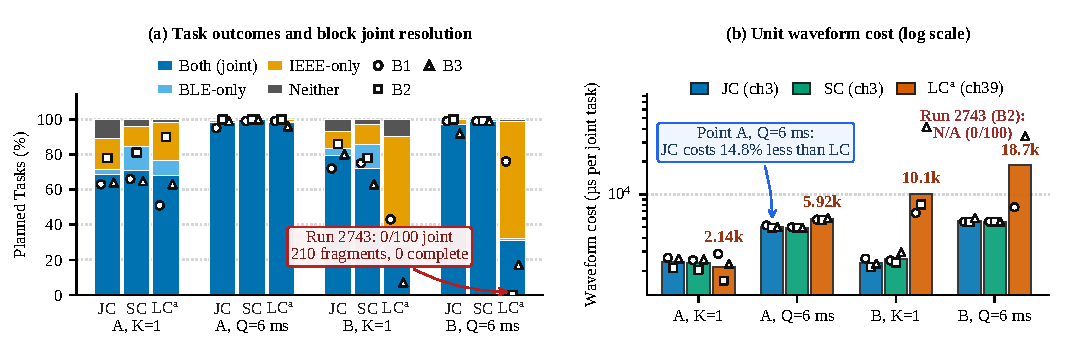
\includegraphics[width=\textwidth]{figures/fig-p4-tradeoff-4p.pdf}
  \caption{Outcomes and unit submitted waveform cost in the 36 wireless runs (\num{3600} planned tasks; at the \SI{6}{ms} cap, $K{=}3/3/4$ at A and $3/3/2$ at B for \modejc{}/\modesc{}/\modelc{}$^{\mathrm{a}}$). (a) Bars pool $300$ tasks; markers show per-block joint resolution (at B under the cap, \modelc{}$^{\mathrm{a}}$ pools $93/300$ from $76,0,17$). (b) Bars divide pooled submitted cost by pooled joint successes (run 2743 is \texttt{N/A} at $0/100$ individually but enters the pooled \SI{18735.5}{\micro\second}/task). $^{\mathrm{a}}$\ble{} ch39 for \modelc{}, ch3 for \modejc{}/\modesc{}.}
  \label{fig:p4_tradeoff}
\end{figure*}

\emph{Wired capacity, offset, and replay (\texttt{R0}):} All 10 tested branches in Table~\ref{tab:budget} achieved $10/10$ dual-chain recovery, covering complete $26/26$, $52/26$, and $28/32$\,B (\ble{}/\stdfour{}) pairs in one secondary PDU, the \SI{27}{B} direct \modelc{} ceiling, and three-/five-fragment \fragproto{} reassembly. Decoding recorded \ble{} IQ with \texttt{zigbee\_rx.py} recovered $10/10$ \stdfour{} commands per run at Points A, B, and C within one \SI{0.25}{\micro\second} sample (\SI{4}{Msps}) of $400{+}8b\,\si{\micro\second}$ (Table~\ref{tab:budget}), verifying intra-packet placement on one clock rather than cross-device synchronization. Deterministic fault injection on recorded streams passed $7/7$ \fragproto{} and $4/4$ state-machine checks (synthetic offline replay).

\emph{Wireless cost and joint resolution (\texttt{R1}):} All 36 P4 runs passed completeness, zero-overflow, and zero-clipping gates (Table~\ref{tab:p4_main}, Figure~\ref{fig:p4_tradeoff}). At short unfragmented Point~A $(0,0)$, \modelc{} has the lowest single-attempt proxy (\SI{1456} vs.\ \SI{1648}{\micro\second}). At $K{=}1$, joint resolution is similar across modes ($204\text{--}212/300$), giving \modelc{} the lowest pooled unit cost (\SI{2141.2} vs.\ \SI{2332.1} for \modesc{} and \SI{2411.7}{\micro\second}/task for \modejc{}). Under $Q{=}\SI{6000}{\micro\second}$, all three near saturation ($294\text{--}299/300$), but open-loop \modelc{} always spends a fourth attempt ($K{=}4$) whereas $K{=}3$ saturates \modejc{} and \modesc{}, flipping unit cost to \SI{5044.9} (\modejc{}, $-14.8\%$) and \SI{4960.5}{\micro\second}/task (\modesc{}, $-16.2\%$) vs.\ \SI{5922.7}{\micro\second}/task (\modelc{}; Figure~\ref{fig:p4_tradeoff}b).

At fragmented Point~B $(26,0)$, \modejc{} and \modesc{} carry the \SI{52}{B} \ble{} record in one secondary PDU (\SI{1856}{\micro\second}/attempt, $K{=}3$ under $Q$), whereas \modelc{} requires five \fragproto{} fragments ($6$ bursts, \SI{2904}{\micro\second}/attempt, $K{=}2$ under $Q$). Across all three blocks, higher joint resolution is observed for ch3 \modejc{} than ch39 \modelc{}: $238/300$ vs.\ $86/300$ at $K{=}1$ (mean $+50.67$\,pp, 95\% $t$-CI $[-4.00,+105.34]$\,pp, unit cost $-76.9\%$) and $291/300$ vs.\ $93/300$ under $Q{=}\SI{6000}{\micro\second}$ (mean $+66.00$\,pp, CI $[-31.58,+163.58]$\,pp, unit cost $-69.4\%$; $7$ of $93$ \modelc{} successes paired cross-slot receptions). Both $\text{df}{=}2$ intervals cross zero, precluding significance claims, and ch3 vs.\ ch39 restricts conclusions to the tested encapsulation-and-channel pair. In Block~2 run 2743 (\modelc{}, $Q{=}\SI{6000}{\micro\second}$), \stdfour{} decoded $98/100$ tasks and \ble{} received $210$ valid fragments across $200$ attempts yet completed $0/100$ records (run unit cost \texttt{N/A}, while its submitted cost enters the pooled numerator); similarly, Block~3 runs 2761 and 2764 received $306$ and $615$ valid fragments but reassembled only $9$ and $19$ records ($7/100$ and $17/100$ joint tasks). Logs cannot isolate physical loss causes, and modeling completion as $p^5$ assumes independent and identically distributed (i.i.d.) fragment reception.

On identical channels (ch3/ch12), all four $\modejc{}-\modesc{}$ CIs cross zero (means $-2.33$ to $+7.33$\,pp), showing neither a consistent joint-resolution gain nor statistical equivalence. Descriptively at $K{=}1$, \modejc{} yields fewer unilateral \texttt{ble\_only} and more simultaneous \texttt{neither} outcomes than \modesc{} ($9/300$ and $33/300$ vs.\ $42/300$ and $12/300$ at A; $12/300$ and $21/300$ vs.\ $41/300$ and $8/300$ at B). Its confirmed co-channel benefit over \modesc{} is cutting bursts per attempt from $3$ to $2$ at equal single-attempt waveform duration alongside the $400{+}8b\,\si{\micro\second}$ offset.

\emph{Fixed-secondary timing and disconnect recovery (\texttt{R0}):} Three $300$-slot Point~B \modejc{} runs ($6$ tasks at $K{=}3$ plus $282$ equal-length \texttt{0x10} updates; post-transmission tail \texttt{stale} separated) test slot-timing availability. In the undisturbed run, joint resolution is $6/6$, held-out probe coverage is $24/24$ per side ($0$ loss events, recovery \texttt{N/A (0/0)}), and the median and 95th percentile (P95) of the absolute local IQ prediction error are $0.223/0.318$\,ms (\ble{}) and $0.129/0.295$\,ms (\stdfour{}). Across two manual unilateral feeder disconnections (\ble{} in run 2716 and \stdfour{} in run 2717), each undisturbed side keeps $24/24$ coverage and \texttt{N/A (0/0)} recovery, while each disrupted side covers $19/24$ probes, resolves $5/6$ joint tasks, and recovers $1/1$ in-schedule (disrupted-side median/P95 errors $0.242/0.395$\,ms and $0.134/0.336$\,ms; \texttt{stale}-to-\texttt{tracking} takes \SI{23.0}{s} and \SI{24.0}{s} on the disrupted receiver's local IQ index, including \SI{7.0}{s} and \SI{9.0}{s} of $8$-packet reacquisition training). In all three runs, $0/6$ planned tasks met the software timed-processing check under uncalibrated external RF bounds; these local errors are not ranked against X-Sync~\cite{hofmann2021xsync}.
